This section describes the alignment of layers and superlayers within
DT chambers, using local information only.  Tracking data are combined
with physical measurements performed when the chambers were
constructed to resolve ambiguities between alignment and
track-fitting.  The chamber geometry obtained by these methods is an
important part of the global alignment described in a later section.

\subsection{Algorithm for General DT Layer Alignment}
\label{sec:standdt_general}

The tracks and physical survey data were merged into a consistent
geometry with a method based on the Millepede algorithm of
V.~Blobel~\cite{ref:Millepede}.  The basic idea behind this algorithm is
to define a $\chi^2$ with contributions from all sources: alignment,
track residuals, and survey residuals, and then minimize the $\chi^2$,
allowing all parameters to float.

Alignment corrections are represented by a vector with 6 parameters
per alignable (layers, superlayers, and in a later section, the
chambers themselves).  These are $\delta_x^i$, $\delta_y^i$,
$\delta_z^i$, $\delta_{\phi_x}^i$, $\delta_{\phi_y}^i$, and
$\delta_{\phi_z}^i$ with $i$ indexing the alignables.  Varying the
alignment affects residuals, the difference between experimental hits and fitted track
points.  Layers and superlayers measure hit positions in only one
dimension, so the effect of geometric corrections on residuals (${\Delta
x^i_j}^{\mbox{\scriptsize \, geom}}$ on alignable $i$ and track $j$) can
be related to alignment parameters through the following matrix:
\begin{equation}
\left(\begin{array}{c} 
{\Delta x^i_j}^{\mbox{\scriptsize \, geom}} \\
\end{array}\right) = 
\left(\begin{array}{c c c c c c}
-1 & 0 & \frac{dx}{dz} & -y\frac{dx}{dz} & x\frac{dx}{dz} & -y  \\
\end{array}\right)\cdot
\left(\begin{array}{c} 
\delta_x^i \\
\delta_y^i \\
\delta_z^i \\
\delta_{\phi_x}^i \\
\delta_{\phi_y}^i \\
\delta_{\phi_z}^i \\
\end{array}\right)
\label{eqn:dtstand_alignparams}
\end{equation}
for each alignable (where $y$ and $\frac{dx}{dz}$ are the track's $y$ position
and $x$ slope with respect to $z$, in the layer's coordinate system).
Tracks are most sensitive to $\delta_x$, and they have no sensitivity
to $\delta_y$ because the term connecting it to ${\Delta
x}^{\mbox{\scriptsize geom}}$ is zero.  We will henceforth denote the
vector of all alignment parameters as $\vec{\delta}$, and the matrix
connecting them to $\Delta x^{\mbox{\scriptsize geom}}$ as $A$ (the index $i$
is internal).  Expanding equation~\ref{eqn:dtstand_alignparams} to cover all alignables,
\begin{equation}
\left(\begin{array}{c} 
{\Delta x_j}^{\mbox{\scriptsize geom}} \\
\end{array}\right) = A \cdot \vec{\delta} \mbox{.}
\end{equation}

Track-fitting is part of the global minimization, so we must include a
term corresponding to variation the track parameters.  We parameterize
tracks inside of DT chambers as straight lines ($x_0$, $y_0$,
$\frac{dx}{dz}$ and $\frac{dy}{dz}$), since magnetic field lines
mainly follow the yokes between chambers, leaving negligible magnetic
field in the chambers themselves.  The effect of small corrections in
the track parameters on residuals ${\Delta
x^i_j}^{\mbox{\scriptsize \, track}}$ is also linear, and may be
represented by a matrix multiplying the track parameter corrections
\begin{equation}
\left(\begin{array}{c}
{\Delta x^i_j}^{\mbox{\scriptsize \, track}} \\
{\Delta y^i_j}^{\mbox{\scriptsize \, track}} \\
\end{array}\right) =
\left(\begin{array}{c c c c}
1 & 0 & z_i & 0 \\
0 & 1 & 0 & z_i \\
\end{array}\right)\cdot
\left(\begin{array}{c}
{\delta_{x_0}}_j \\
{\delta_{y_0}}_j \\
{\delta_{\frac{dx}{dz}}}_j \\
{\delta_{\frac{dy}{dz}}}_j \\
\end{array}\right)
\label{eqn:dtstand_trackparams}
\end{equation}
in the chamber's coordinate system.  (As a reminder, one-dimensional
$x$ positions in layer coordinates transform to $(0,\mbox{ }x)$ in
two-dimensional chamber coordinates for superlayer~2 and $(x,\mbox{
}0)$ for superlayers~1 and 3, in the absence of alignment
corrections.)  We will denote the corrections to the track parameters
as $\delta \vec{p_j}$ and the matrix connecting them to
$x^{\mbox{\scriptsize track}}$ as $B_j$, such that
Equation~\ref{eqn:dtstand_trackparams} becomes
\begin{equation}
\left(\begin{array}{c}
{\Delta x^i_j}^{\mbox{\scriptsize \, track}} \\
{\Delta y^i_j}^{\mbox{\scriptsize \, track}} \\
\end{array}\right) = B_j \cdot \delta \vec{p_j} \mbox{.}
\end{equation}

The observed residuals $\Delta \vec{x}$ are
\begin{equation}
\Delta \vec{x} = \Delta \vec{x}^{\mbox{\scriptsize \, geom}} + \Delta
\vec{x}^{\mbox{\scriptsize \, track}}
+ \Delta \vec{x}^{\mbox{\scriptsize \, meas}}
\end{equation}
where $\Delta \vec{x}^{\mbox{\scriptsize \, meas}}$ is a random
contribution from measurement error, assumed to be symmetric.  We can
now construct a $\chi^2$ which is minimized when tracks and chamber
geometry are mutually consistent:
\begin{equation}
{\chi^2}^{\mbox{\scriptsize \, track-based}} = \sum_j \left(\Delta \vec{x} - A \cdot \vec{\delta} - B_j \cdot \delta \vec{p_j} \right)^T \, \left({\sigma_{\mbox{\scriptsize resid}_{\mbox{\scriptsize $i$}}}}^2\right)^{-1} \, \left(\Delta \vec{x} - A \cdot \vec{\delta} - B_j \cdot \delta \vec{p_j} \right)
\label{eqn:chi2millepede}
\end{equation}
where ${\sigma_{\mbox{\scriptsize resid}_{\mbox{\scriptsize $i$}}}}^2$
is the covariance matrix of hits (no uncertainty in our track model).
However, ${\chi^2}^{\mbox{\scriptsize \, track-based}}$ cannot be
minimized: the system has more degrees of freedom than
constraints.  Consider, for instance, shearing all layers linearly in
$x$; this non-rigid deformation of the chamber leaves
${\chi^2}^{\mbox{\scriptsize \, track-based}}$ invariant because
fitted tracks compensate with $\frac{dx}{dz}$.  We therefore must
augment it with external data to yield a meaningful alignment.

\subsubsection{Quality Control Measurements}

As the DT chambers were being built, the positions of the wire
end-pins were measured and recorded~\cite{ref:QC}.  Local $\delta_x^i$
corrections can be determined from an average of the measurements over
layers.  Typical (RMS) corrections are 100~$\mu$m, with an uncertainty of 30--40~$\mu$m.  These measurements only constrain the
relative positions of layers within each superlayer, not the
superlayers relative to one another, because each superlayer was built
separately.

\subsubsection{Photogrammetry Measurements}

After superlayers were assembled into chambers, the position and
orientation of the superlayers were measured by photogrammetry (a
photograph of reflective targets at known points on the superlayer, in
a coordinate system defined by references at their
corners~\cite{ref:Survey}).  These measurements constrain superlayers
relative to one another, but not the layers inside).

Typical corrections are 200~$\mu$m for $\delta_x$ and $\delta_y$, with
150~$\mu$rad for rotations.  The $\delta_z$ corrections were 1--1.5~mm
because of a layer of glue not included in the design description.  We
take special care to cross-check these $\delta_z$ parameters
independently with tracks before applying the correction.

\subsubsection{Combination}

To include survey measurements into the global alignment fit, we need
a term to describe the effect of alignment corrections
$\vec{\delta^i}$ on the positions of the survey's control points
(nominally at $x_k$, $y_k$, $z_k$).  This term is
\begin{equation}
{\Delta \vec{x^i_k}}^{\mbox{\scriptsize \, points}} =
\left(\begin{array}{c c c c c c}
1 & 0 & 0 & y_k & z_k & 0 \\
0 & 1 & 0 & -x_k & 0 & z_k \\
0 & 0 & 1 & 0 & -x_k & -y_k \\
\end{array}\right) \cdot
\vec{\delta^i}
\end{equation}
and we denote the matrix for all control points on all alignables as
$C$ (alignable index $i$ and survey point index $k$ are internal).
This matrix is constructed in such a way as to internally account for
the fact that some measurements are relative differences, rather than
absolute coordinates.  The $\chi^2$ of survey measurements is
\begin{equation}
{\chi^2}^{\mbox{\scriptsize \, survey}} = \left({\Delta \vec{x}}^{\mbox{\scriptsize \, survey}} - C \cdot \vec{\delta} \right)^T \, \left({\sigma_{\mbox{\scriptsize survey}}}^2\right)^{-1} \, \left({\Delta \vec{x}}^{\mbox{\scriptsize \, survey}} - C \cdot \vec{\delta} \right)
\end{equation}
where ${\Delta \vec{x}}^{\mbox{\scriptsize \, survey}}$ are the measured positions
from survey and photogrammetry, and ${\sigma_{\mbox{\scriptsize
survey}}}^2$ is their covariance matrix.

Finally, the global chamber position can never be determined from
local information, so translations and rotations of the whole chamber
are fixed to zero with Lagrange multipliers $f(\lambda)$.  The final
$\chi^2$ is
\begin{equation}
\chi^2 = {\chi^2}^{\mbox{\scriptsize \, track-based}} +
{\chi^2}^{\mbox{\scriptsize \, survey}} + f(\lambda) \mbox{,}
\end{equation}
which we minimize by a straight-forward numerical inversion of the
derivatives matrix, as the number of alignable parameters is not
large.

\begin{figure}
\centering
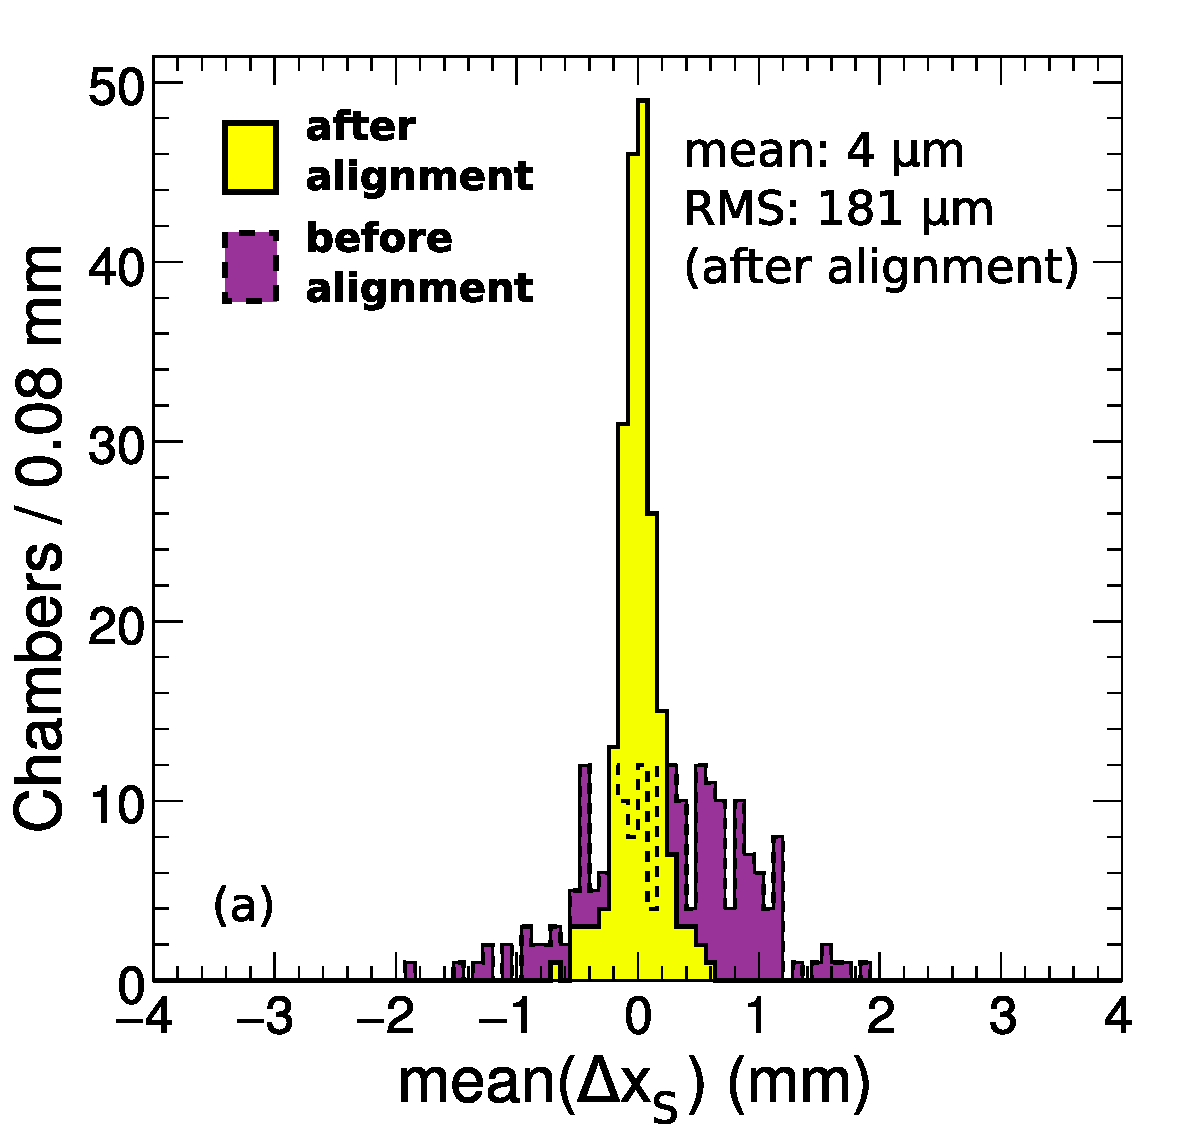
\includegraphics[width=0.5\linewidth]{plots/standalone_dt_alignment/residualsStandaloneAlignment.pdf}
\caption{something \label{fig:residualsStandaloneAlignment}}
\end{figure}

\subsection{Independent Cross-Check of $\delta_z$}
\label{sec:standdt_independent}

As explained above, the largest correction from the design geometry
was in the superlayers' $z$ coordinates, due to a layer of glue not
included in the design description.  To cross-check these
photogrammetry measurements, we determined them from an independent
track-based measurement.

As the displacement under study is between superlayers, track segments
fitted in each superlayer individually are not affected by the
correction.  We can therefore simplify the $\chi^2$ by re-defining
residuals in this case as a difference between single-superlayer track
segments (superlayers~1 and 3 only), extrapolated to a common plane.
The $B_j$ matrix vanishes, leaving us with
\begin{equation}
\chi^2 = \sum_j \left(\Delta \vec{x} - A \cdot \vec{\delta}\right)^T \, \left({\sigma_{\mbox{\scriptsize resid}}}^2\right)^{-1} \, \left(\Delta \vec{x} - A \cdot \vec{\delta}\right)
\end{equation}
where ${\sigma_{\mbox{\scriptsize resid}}}^2$ is the covariance matrix
for these new residuals.  We further simplify the alignment by only
allowing $\delta_x$, $\delta_z$, and $\delta_{\phi_y}$ to float, as
these are the parameters that can be determined purely from track
segments in one-dimensional measurement devices.  The alignment
derivatives matrix $A$ for each chamber is reduced to
\begin{equation}
\left(\begin{array}{c} 
{\Delta x^i_j}^{\mbox{\scriptsize \, geom}} \\
\end{array}\right) = 
\left(\begin{array}{c c c c c c}
-1 & \frac{dx}{dz} & x\frac{dx}{dz}  \\
\end{array}\right)\cdot
\left(\begin{array}{c} 
\delta_x^i \\
\delta_z^i \\
\delta_{\phi_y}^i \\
\end{array}\right) \mbox{.}
\end{equation}
A geometric interpretation of the $\delta_z$ term is given in
Figure~\ref{fig:extrapolation}.  With these simplifications, it is
possible to align superlayers purely with track-based data.

\begin{figure}
  \begin{center}
  \subfigure[Interpretation of $\Delta x^{\mbox{\scriptsize geom}} = \frac{dx}{dz} \delta_z$.]{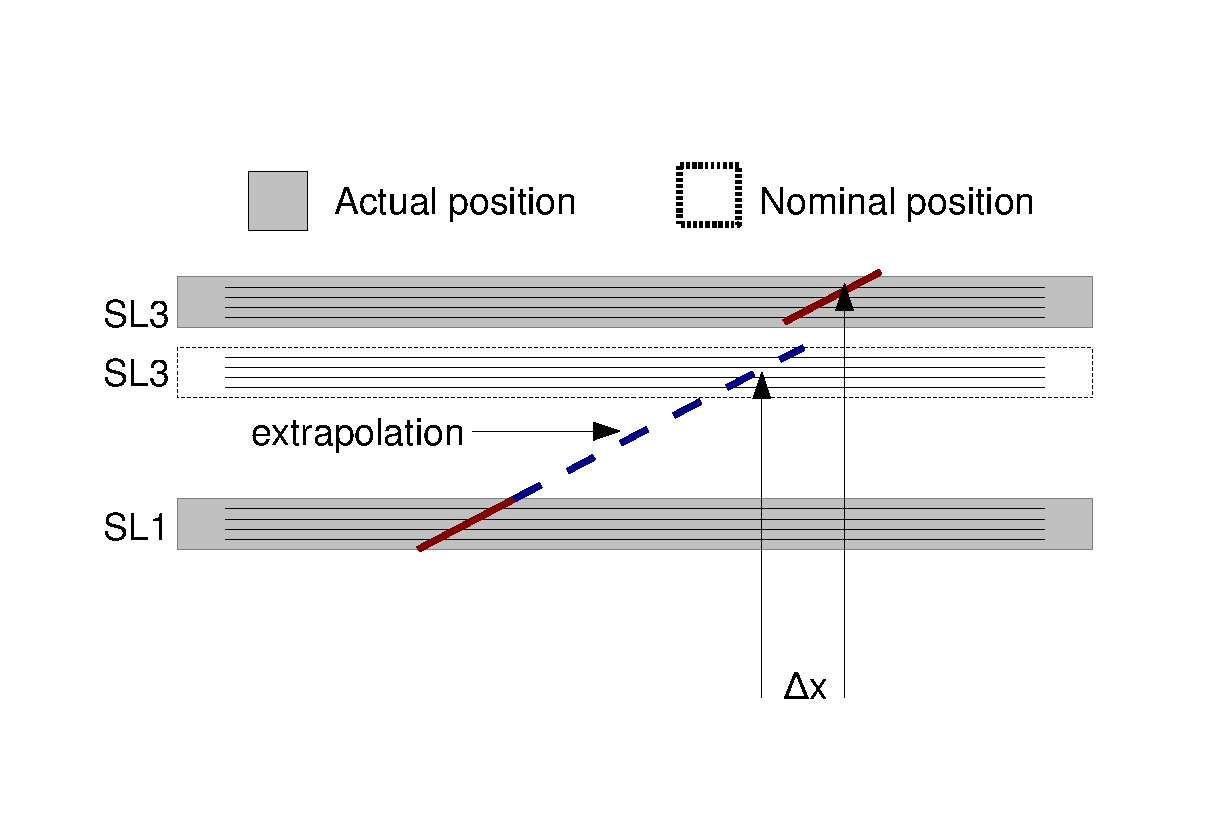
\includegraphics[width=0.45\linewidth]{plots/standalone_dt_alignment/internalThickness.pdf} \label{fig:extrapolationa}}
  \subfigure[A typical $\delta_z$ displacement, observed as a slope in $\Delta x$ versus $\frac{dx}{dz}$.]{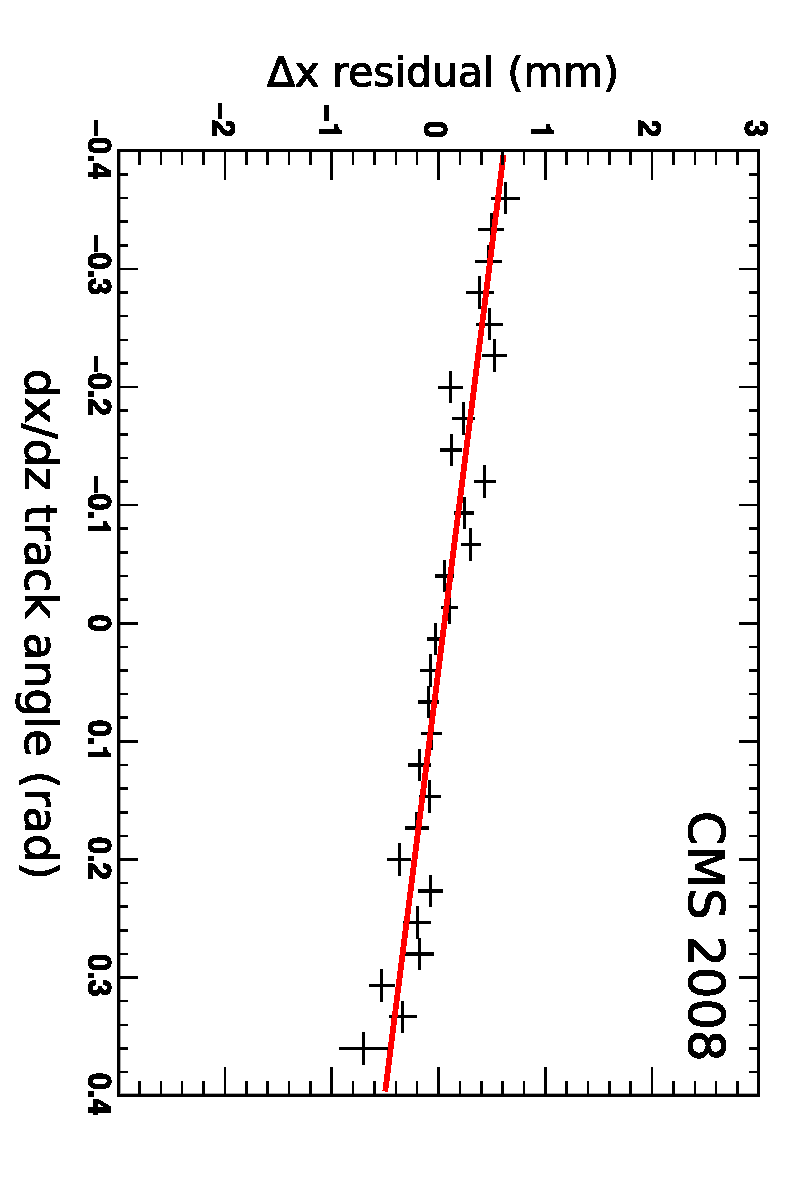
\includegraphics[height=0.45\linewidth, angle=90]{plots/standalone_dt_alignment/xphi014.pdf} \label{fig:slopetracks}}
  \end{center}
  \caption{Measuring $\delta_z$ with tracks only. \label{fig:extrapolation}}
\end{figure}

The $\delta_z$ corrections from survey (photogrammetry), this
track-based method, and their differences are plotted in
Figure~\ref{fig:surveyvstracks}, revealing independent agreement in
non-negligible corrections.  Typical discrepancies are 580~$\mu$m (RMS
and Gaussian width) in $\delta_z$, while the size of the corrections
range from 1 to 2~mm (thicker glue was used in station~1).  The
$\delta_x$ and $\delta_{\phi_y}$ corrections were also in agreement,
but they were negligible (80~$\mu$m and 50~$\mu$rad, respectively).

\begin{figure}
  \begin{center}
  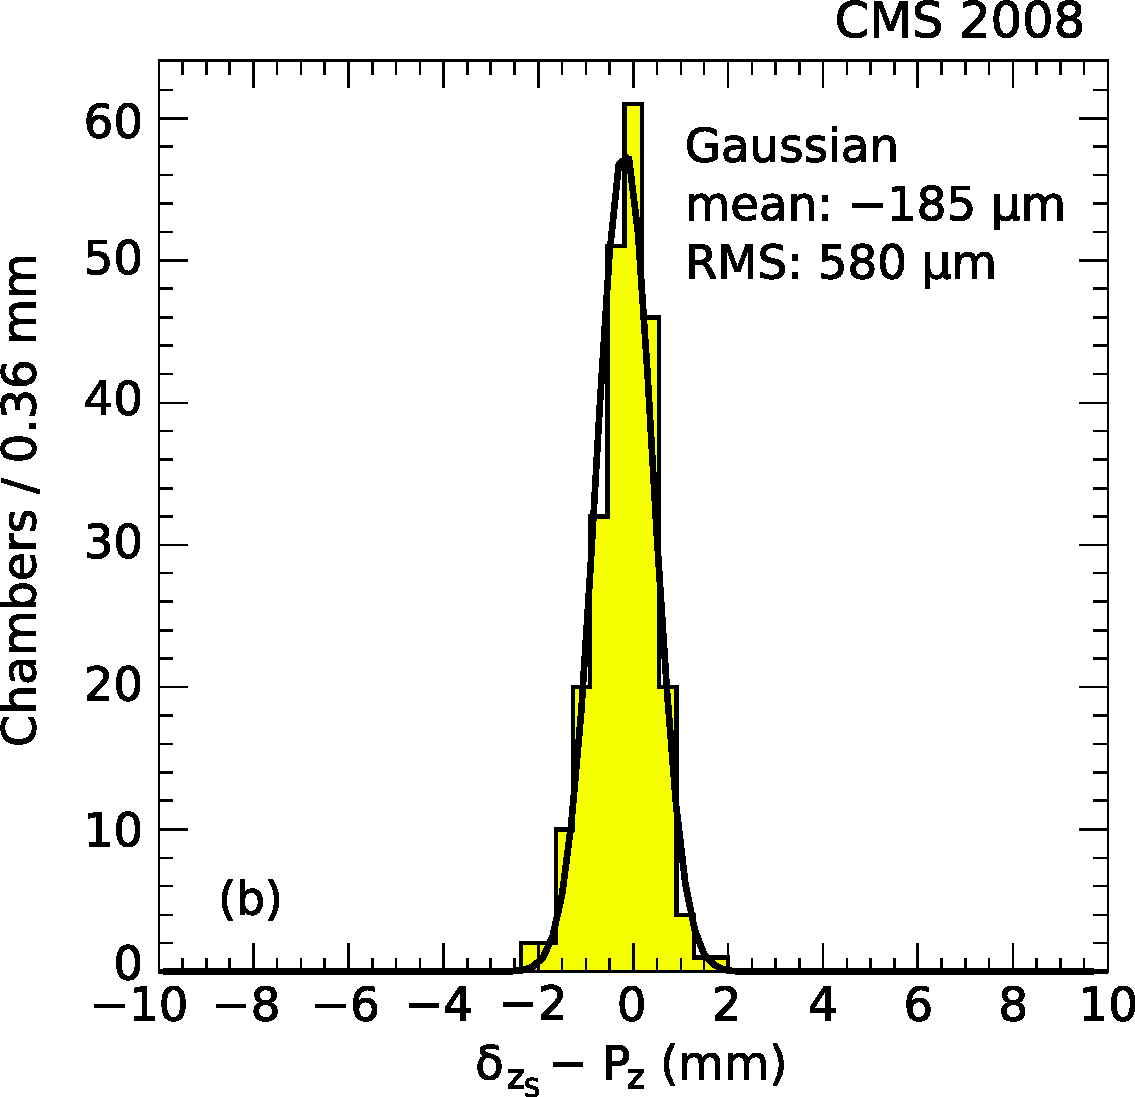
\includegraphics[width=0.5\linewidth]{plots/standalone_dt_alignment/DiffereceancesAllSurveyTracks.pdf}
  \end{center}
  \caption{Comparison of survey and track-based alignment of $\delta_z$ of superlayers in DT chambers.  Each entry in this histogram is a $\delta_z$ measurement for one chamber, with the three distributions corresponding to survey (photogrammetry) only, tracks only, and the chamber-by-chamber difference between survey and tracks. \label{fig:surveyvstracks}}
\end{figure}

The internal DT geometry used in the global alignment was determined
by the combined fit described in subsection~\ref{sec:standdt_general}
with $\delta_z$ fixed, followed by corrections from the tracks-only
method described above.  It therefore incorporates all available
information except that which is reserved for cross-checking the
sources.
